\newpage
\subsection{Forget Password Page}\hfill 

%For the main pages put a mockup and describe it in detail.

%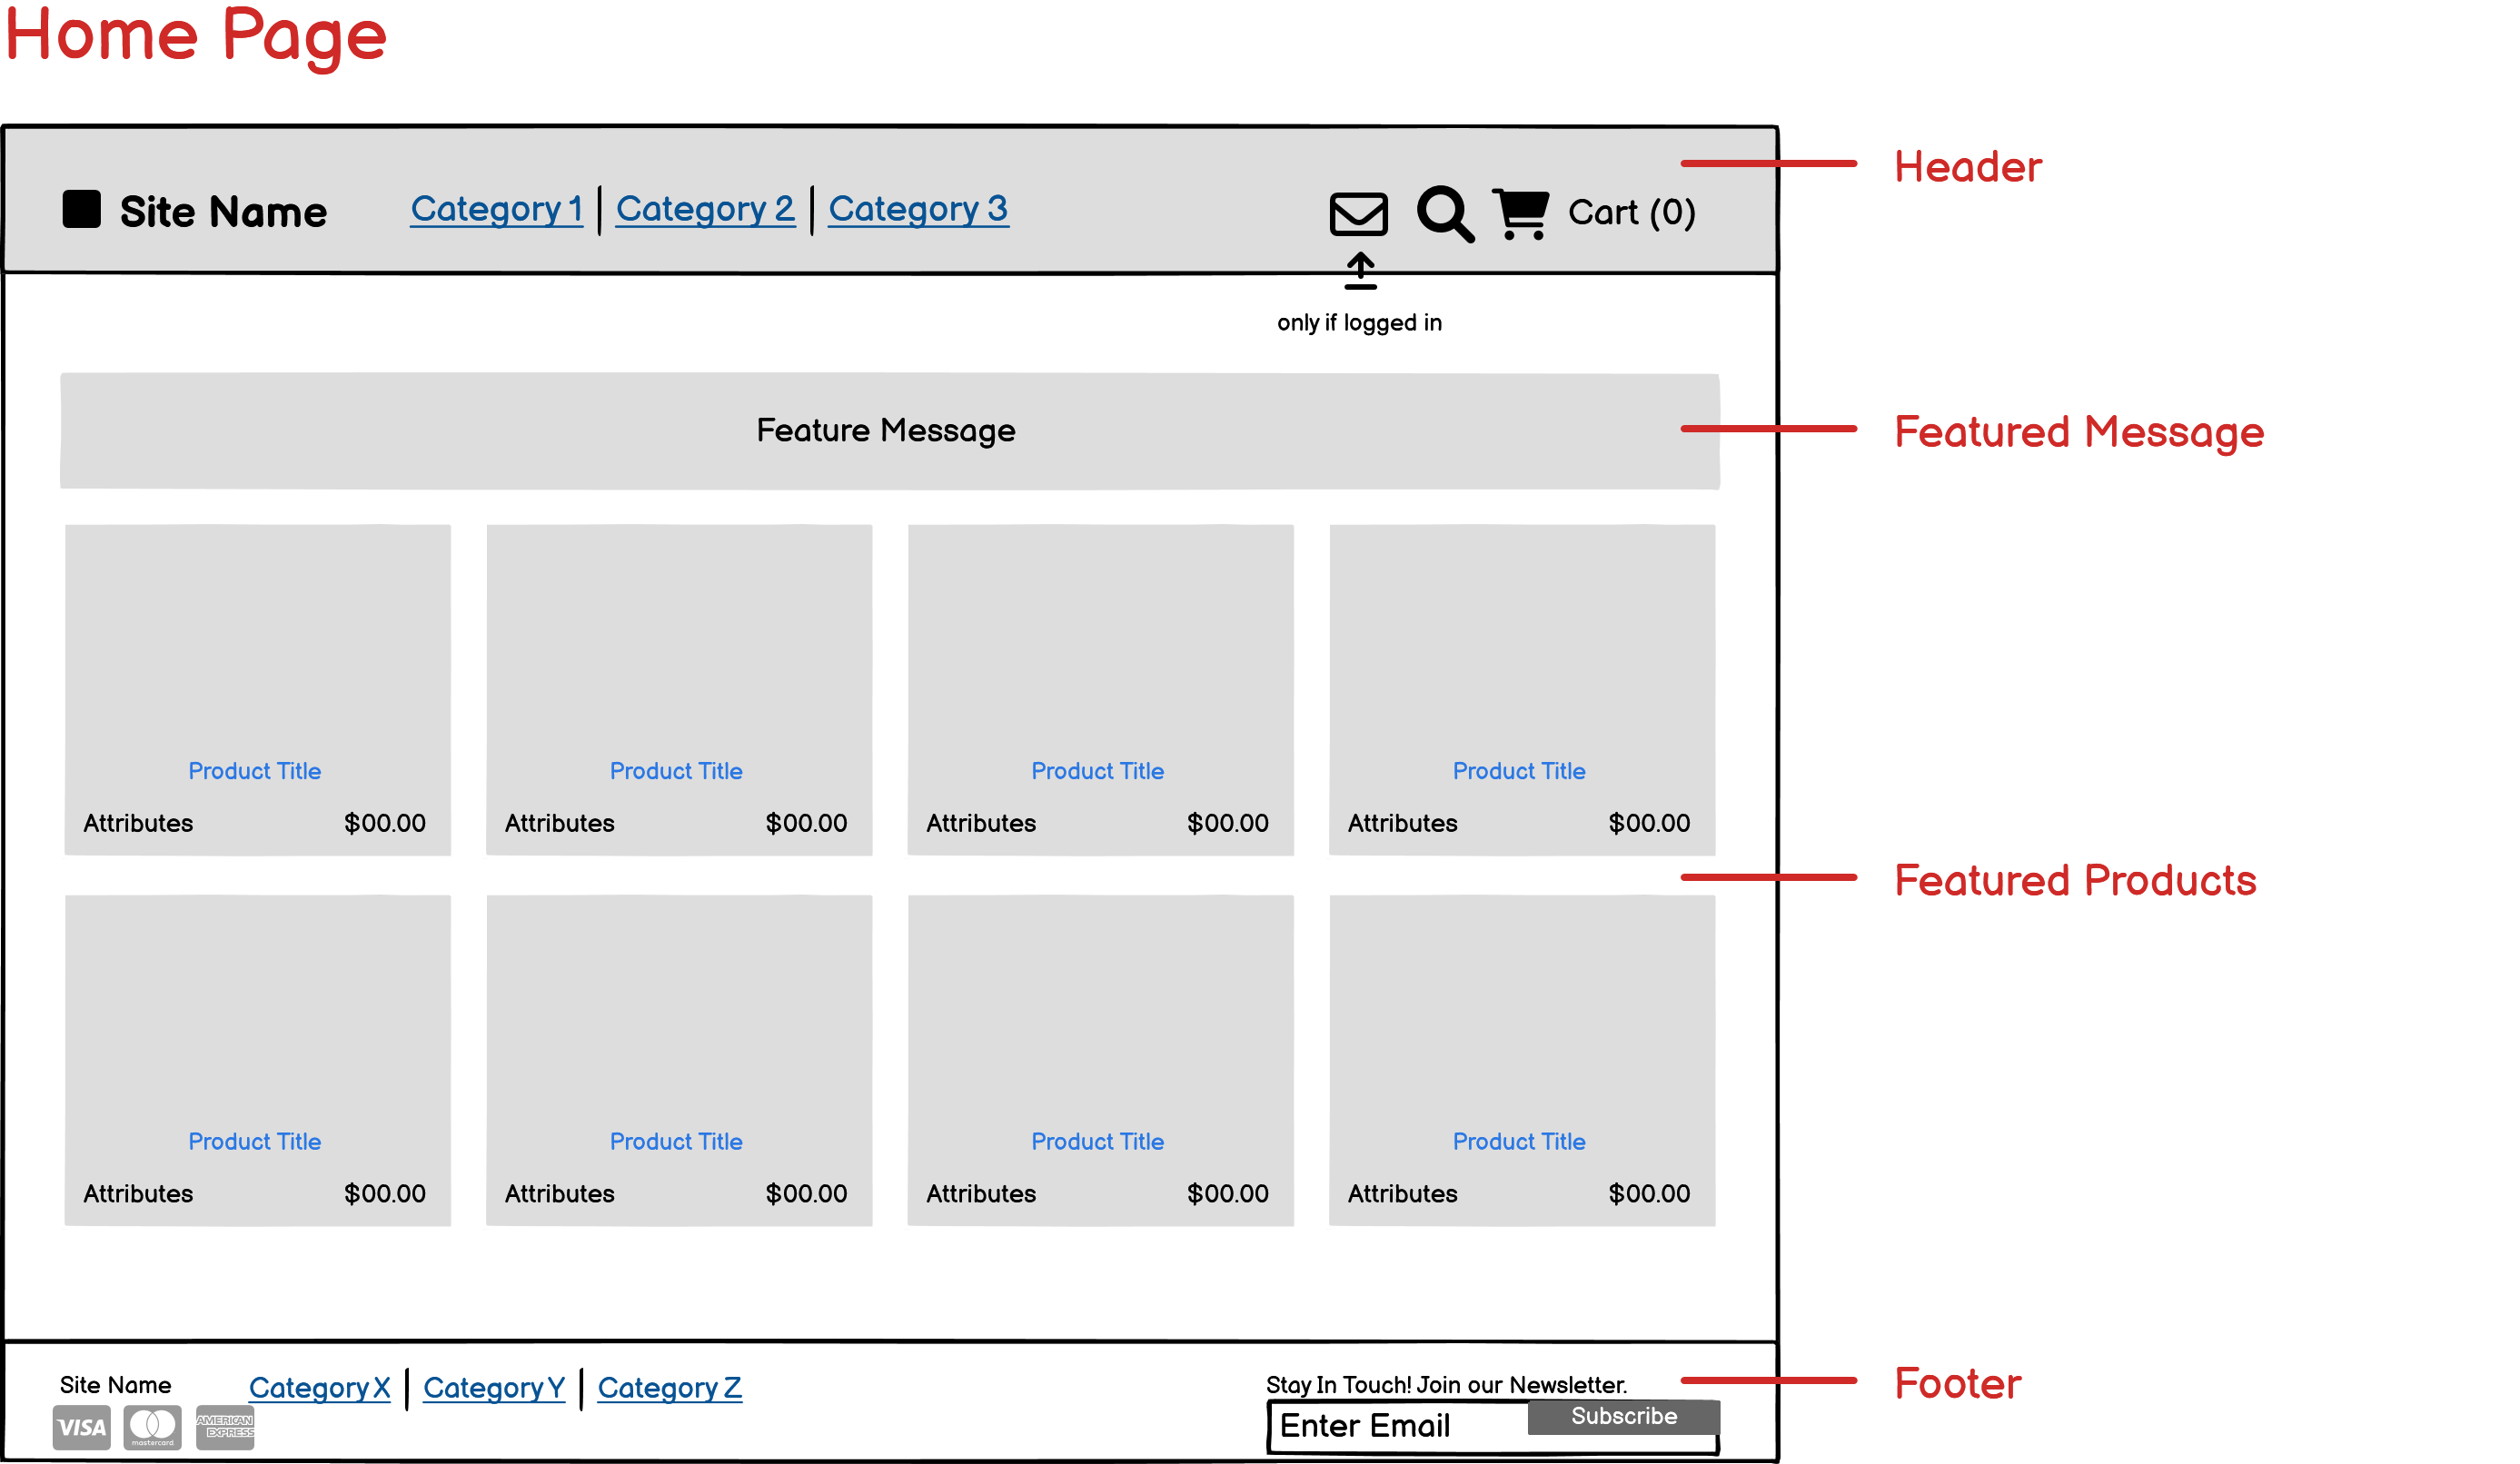
\includegraphics[scale=0.5]{logos/Images/pages/Home Page.png}

\begin{figure}[h]
    \centering
    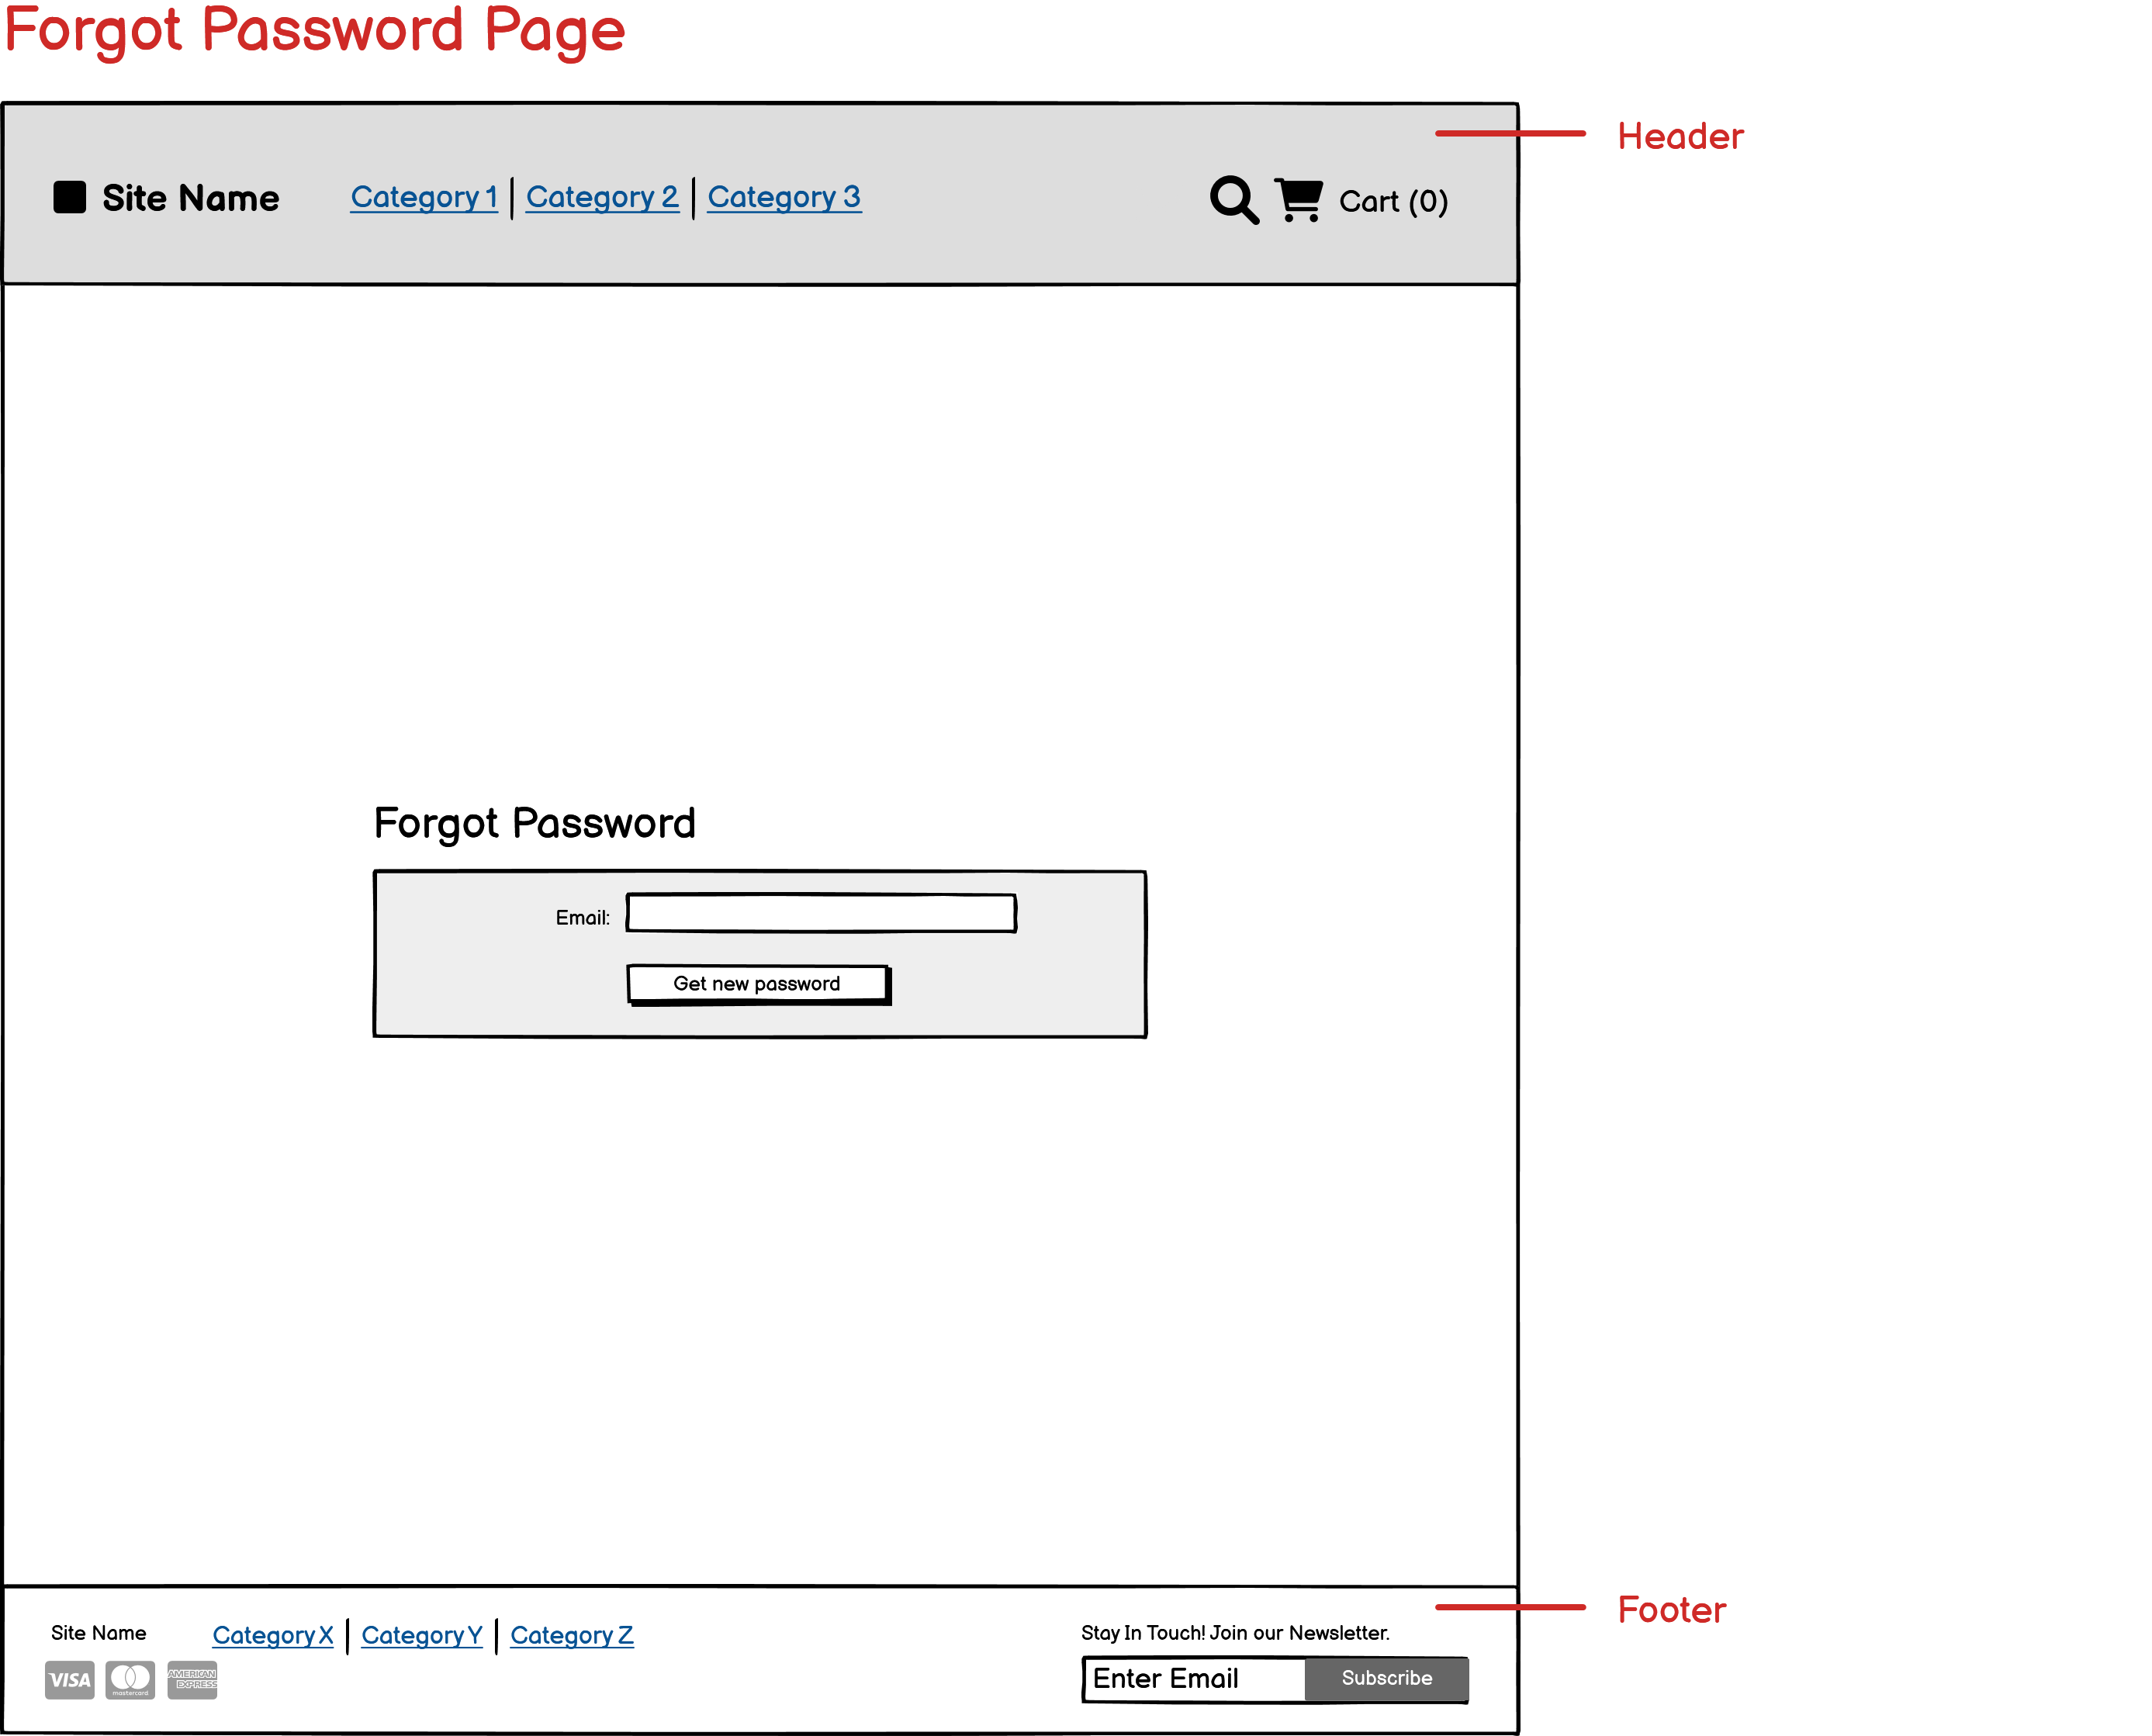
\includegraphics[scale=0.4]{logos/Images/pages/Forget Password Page.png}
    \caption{Forget Password Page}
    \label{fig:my_label}
\end{figure}
\hfill \break
In case a user forgets his password, this website provides a password reset option. In order to reset the password, the user only needs to enter their email address associated with their account.\\\\
Once the user enters their email address, an email will be sent to that address with a password reset link. The user can then click on the link and create a new password to access their account.\\\\
Using the email address as the only information needed when resetting the password has the advantage of making it easy and quick to reset the password. The user does not need to remember different information or perform special steps to reset his password.